\documentclass[a4paper, 14pt]{extarticle}

\usepackage{cmap}
\usepackage[T2A]{fontenc}
\usepackage[utf8]{inputenc}
\usepackage[english, russian]{babel}
\usepackage{amsmath}
\usepackage{subcaption}
\usepackage{graphicx}
\usepackage{float}
\usepackage{hyperref}

\usepackage[left=3cm, right=1.5cm, top=2cm, bottom=2cm]{geometry}
\usepackage{setspace}
\onehalfspacing 

\usepackage{indentfirst}
\setlength{\parindent}{1.25cm} 
\setlength{\emergencystretch}{3em}
\usepackage[expansion=false,protrusion=false,nopatch=footnote]{microtype}

\usepackage{tocloft}
\addto\captionsrussian{\renewcommand{\contentsname}{СОДЕРЖАНИЕ}}
\renewcommand{\cfttoctitlefont}{\hfill\normalfont}
\renewcommand{\cftaftertoctitle}{\hfill\vspace{\baselineskip}}
\renewcommand{\cftsecdotsep}{\cftdotsep}

\begin{document}

\begin{titlepage}
    \begin{center}
        Министерство науки и высшего образования Российской Федерации\\
        Федеральное государственное автономное образовательное учреждение высшего образования\\
        «Санкт-Петербургский политехнический университет Петра Великого»\\
        
        \textbf{Физико-механический институт}\\
        \textbf{Высшая школа прикладной математики и вычислительной физики}
    \end{center}

    \vfill
    
    \begin{center}
        \textbf{Отчёт по лабораторной работе \textnumero~ 3\\[0.5cm]}
        \textbf{Боксплот Тьюки и анализ выбросов\\}
        по дисциплине <<Математическая статистика>>
    \end{center}

    \vfill

    \hfill
    \begin{minipage}{0.45\textwidth}
        \textbf{Выполнил студент гр. 5030102/30202:}\\
        Шильдт Д.С.\\[0.5cm]
        \textbf{Преподаватель:}\\ 
        Баженов А.Н.
    \end{minipage}

    \vfill

    \begin{center}
        Санкт-Петербург\\2026
    \end{center}
\end{titlepage}

\setcounter{page}{2}

\tableofcontents
\newpage

\section{Постановка задачи}

\textbf{Цели и задачи работы:}
\begin{itemize}
    \item Научиться применять боксплот Тьюки в обработке и анализе одномерных распределений.
    \item Проанализировать, как размер выборки влияет на долю отсеиваемых аномальных значений.
\end{itemize}

\textbf{Задание:}
Для пяти исследуемых распределений (Нормальное $N(0, 1)$, Коши $C(0, 1)$, Лапласа $L(0, 1/\sqrt{2})$, Пуассона $P(5)$ и Равномерное $U(-\sqrt{3}, \sqrt{3})$) необходимо выполнить следующие шаги:
\begin{enumerate}
    \item Сгенерировать выборки объемом $n \in \{20, 100\}$. Построить боксплот Тьюки.
    \item  Определить долю выбросов экспериментально: для каждого распределения сгенерировать 1000 выборок заданного объёма, вычислить среднюю долю выбросов.
\end{enumerate}

Практическая доля выбросов в выборке ситается как отношение количества выбросов к
количеству всех элементов в выборке. В данной работе необходимо посчитать среднюю
долю выбросов, сгнерировав выборку 1000 раз.

\section{Теоретическая часть}

Для графического анализа одномерных выборок и выявления аномальных значений применяется диаграмма боксплот Тьюки. Границами центрального прямоугольника выступают нижняя $z_{1/4}$ и верхняя $z_{3/4}$ выборочные квартили. Длина ящика соответствует интерквартильной широте $IQR = z_{3/4} - z_{1/4}$.

Левый и правый «усы» определяют границы нормального (неаномального) разброса данных и вычисляются по формулам:
\begin{equation}
    X_1^r = z_{1/4} - 1.5 \cdot IQR
\end{equation}
\begin{equation}
    X_2^r = z_{3/4} + 1.5 \cdot IQR
\end{equation}

Любой элемент выборки $x_i$, удовлетворяющий условию $x_i < X_1^r$ или $x_i > X_2^r$, классифицируется как выброс. Доля выбросов рассчитывается как отношение количества таких аномальных элементов к общему объему выборки $n$.
\section{Реализация}

\subsection{Язык программирования и среда}
    \begin{itemize}
        \item \textbf{Используемый язык:} Python 3.14.2
        \item \textbf{Используемая среда разработки:} Visual Studio Code
    \end{itemize}

\subsection{Используемые библиотеки}
    \begin{itemize}
        \item \textbf{numpy} --- использовалась для работы с массивами, вычисления квартилей и обработки результатов моделирования.
        \item \textbf{scipy} --- использовалась для генерации выборок из теоретических распределений (\texttt{norm}, \texttt{cauchy}, \texttt{laplace}, \texttt{poisson}, \texttt{uniform}).
        \item \textbf{matplotlib} --- использовалась для построения боксплотов Тьюки и столбчатой диаграммы средней доли выбросов.
        \item \textbf{pathlib} --- использовалась для автоматического создания каталогов и сохранения итоговых графиков и CSV-файла.
    \end{itemize}

\subsection{Суть реализованных методов}

\begin{itemize}
    \item \texttt{getDistributionConfigs()} — формирует единый список конфигураций исследуемых распределений (название, идентификатор файла и функция-генератор выборки).
    \item \texttt{tukeyBounds(sample)} — вычисляет границы выбросов по правилу Тьюки $X_1^r$ и $X_2^r$ через выборочные квартили и интерквартильную широту $IQR$.
    \item \texttt{outlierShare(sample)} — определяет долю выбросов в одной выборке как отношение количества наблюдений за границами Тьюки к объему выборки.
    \item \texttt{meanOutlierShare(generator, sample\_size, repeats, rng)} — реализует серию из 1000 повторов генерации и вычисляет среднюю долю выбросов для каждого распределения и каждого объема выборки $n \in \{20, 100\}$.
    \item \texttt{saveBoxplotFigure(...)} — строит и сохраняет боксплоты Тьюки для объемов $n \in \{20, 100\}$.
    \item \texttt{saveOutlierShareFigure(rows)} — строит итоговую столбчатую диаграмму средних долей выбросов для всех распределений при двух объемах выборки.
    \item \texttt{saveOutlierCsv(rows)} и \texttt{printReport(rows)} — отвечают за экспорт и представление результатов.
\end{itemize}

\section{Результаты}

В ходе работы для каждого исследуемого распределения построены диаграммы Тьюки при объемах выборки $n \in \{20, 100\}$ (рис.~\ref{fig:norm_boxplot}--\ref{fig:uniform_boxplot}). Дополнительно на рис.~\ref{fig:outlier_share} показано сравнение средних долей выбросов по всем распределениям.

Экспериментально определенная средняя доля аномальных значений (выбросов), вычисленная по 1000 независимым повторениям генерации выборок, приведена в таблице \ref{tab:outliers}.

\begin{table}[H]
    \centering
    \caption{Средняя доля выбросов для исследуемых распределений}
    \label{tab:outliers}
    \small
    \resizebox{\textwidth}{!}{%
    \begin{tabular}{|l|c|c|}
        \hline
        \textbf{Распределение} & \textbf{Средняя доля выбросов, $n=20$} & \textbf{Средняя доля выбросов, $n=100$} \\ \hline
        $N(0,1)$ & 0.0185 & 0.0096 \\ \hline
        $C(0,1)$ & 0.1368 & 0.1520 \\ \hline
        $L(0, 1/\sqrt{2})$ & 0.0592 & 0.0623 \\ \hline
        $P(5)$ & 0.0185 & 0.0129 \\ \hline
        $U(-\sqrt{3}, \sqrt{3})$ & 0.0013 & 0.0000 \\ \hline
    \end{tabular}%
    }
\end{table}

\begin{figure}[H]
    \centering
    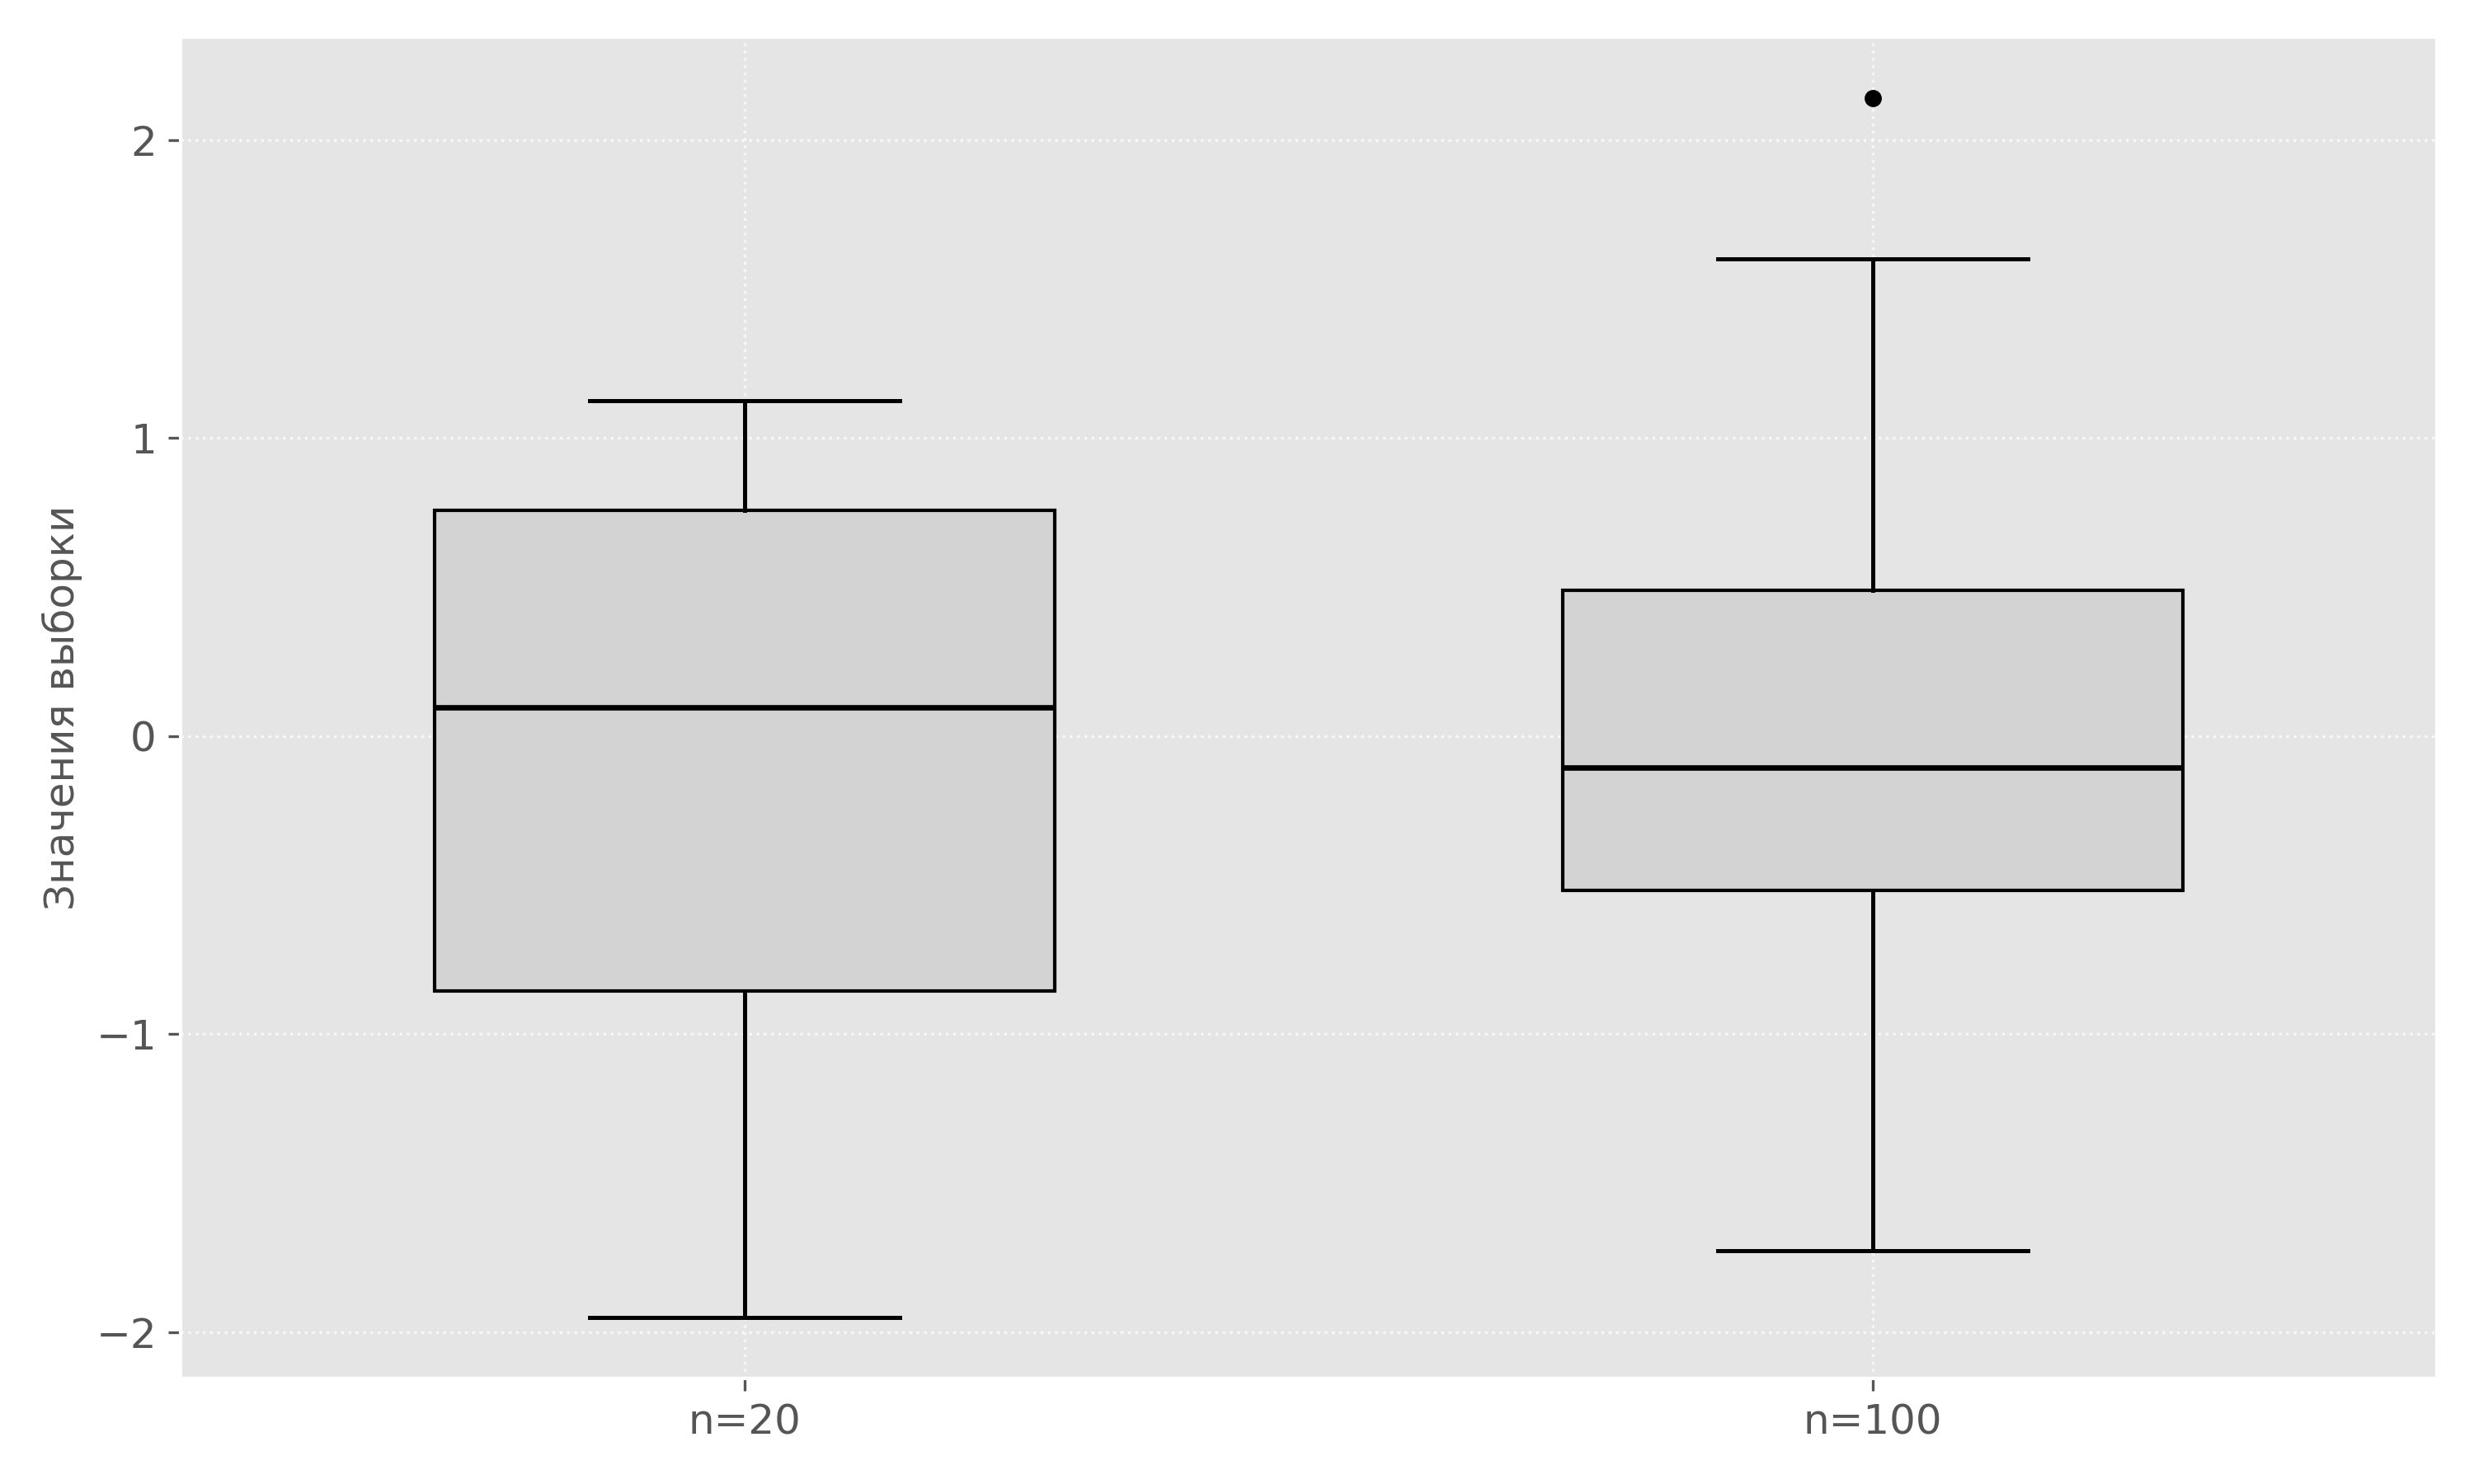
\includegraphics[width=\textwidth]{../figures/norm_boxplot.png}
    \caption{Боксплот Тьюки для нормального распределения $N(0,1)$}
    \label{fig:norm_boxplot}
\end{figure}

\begin{figure}[H]
    \centering
    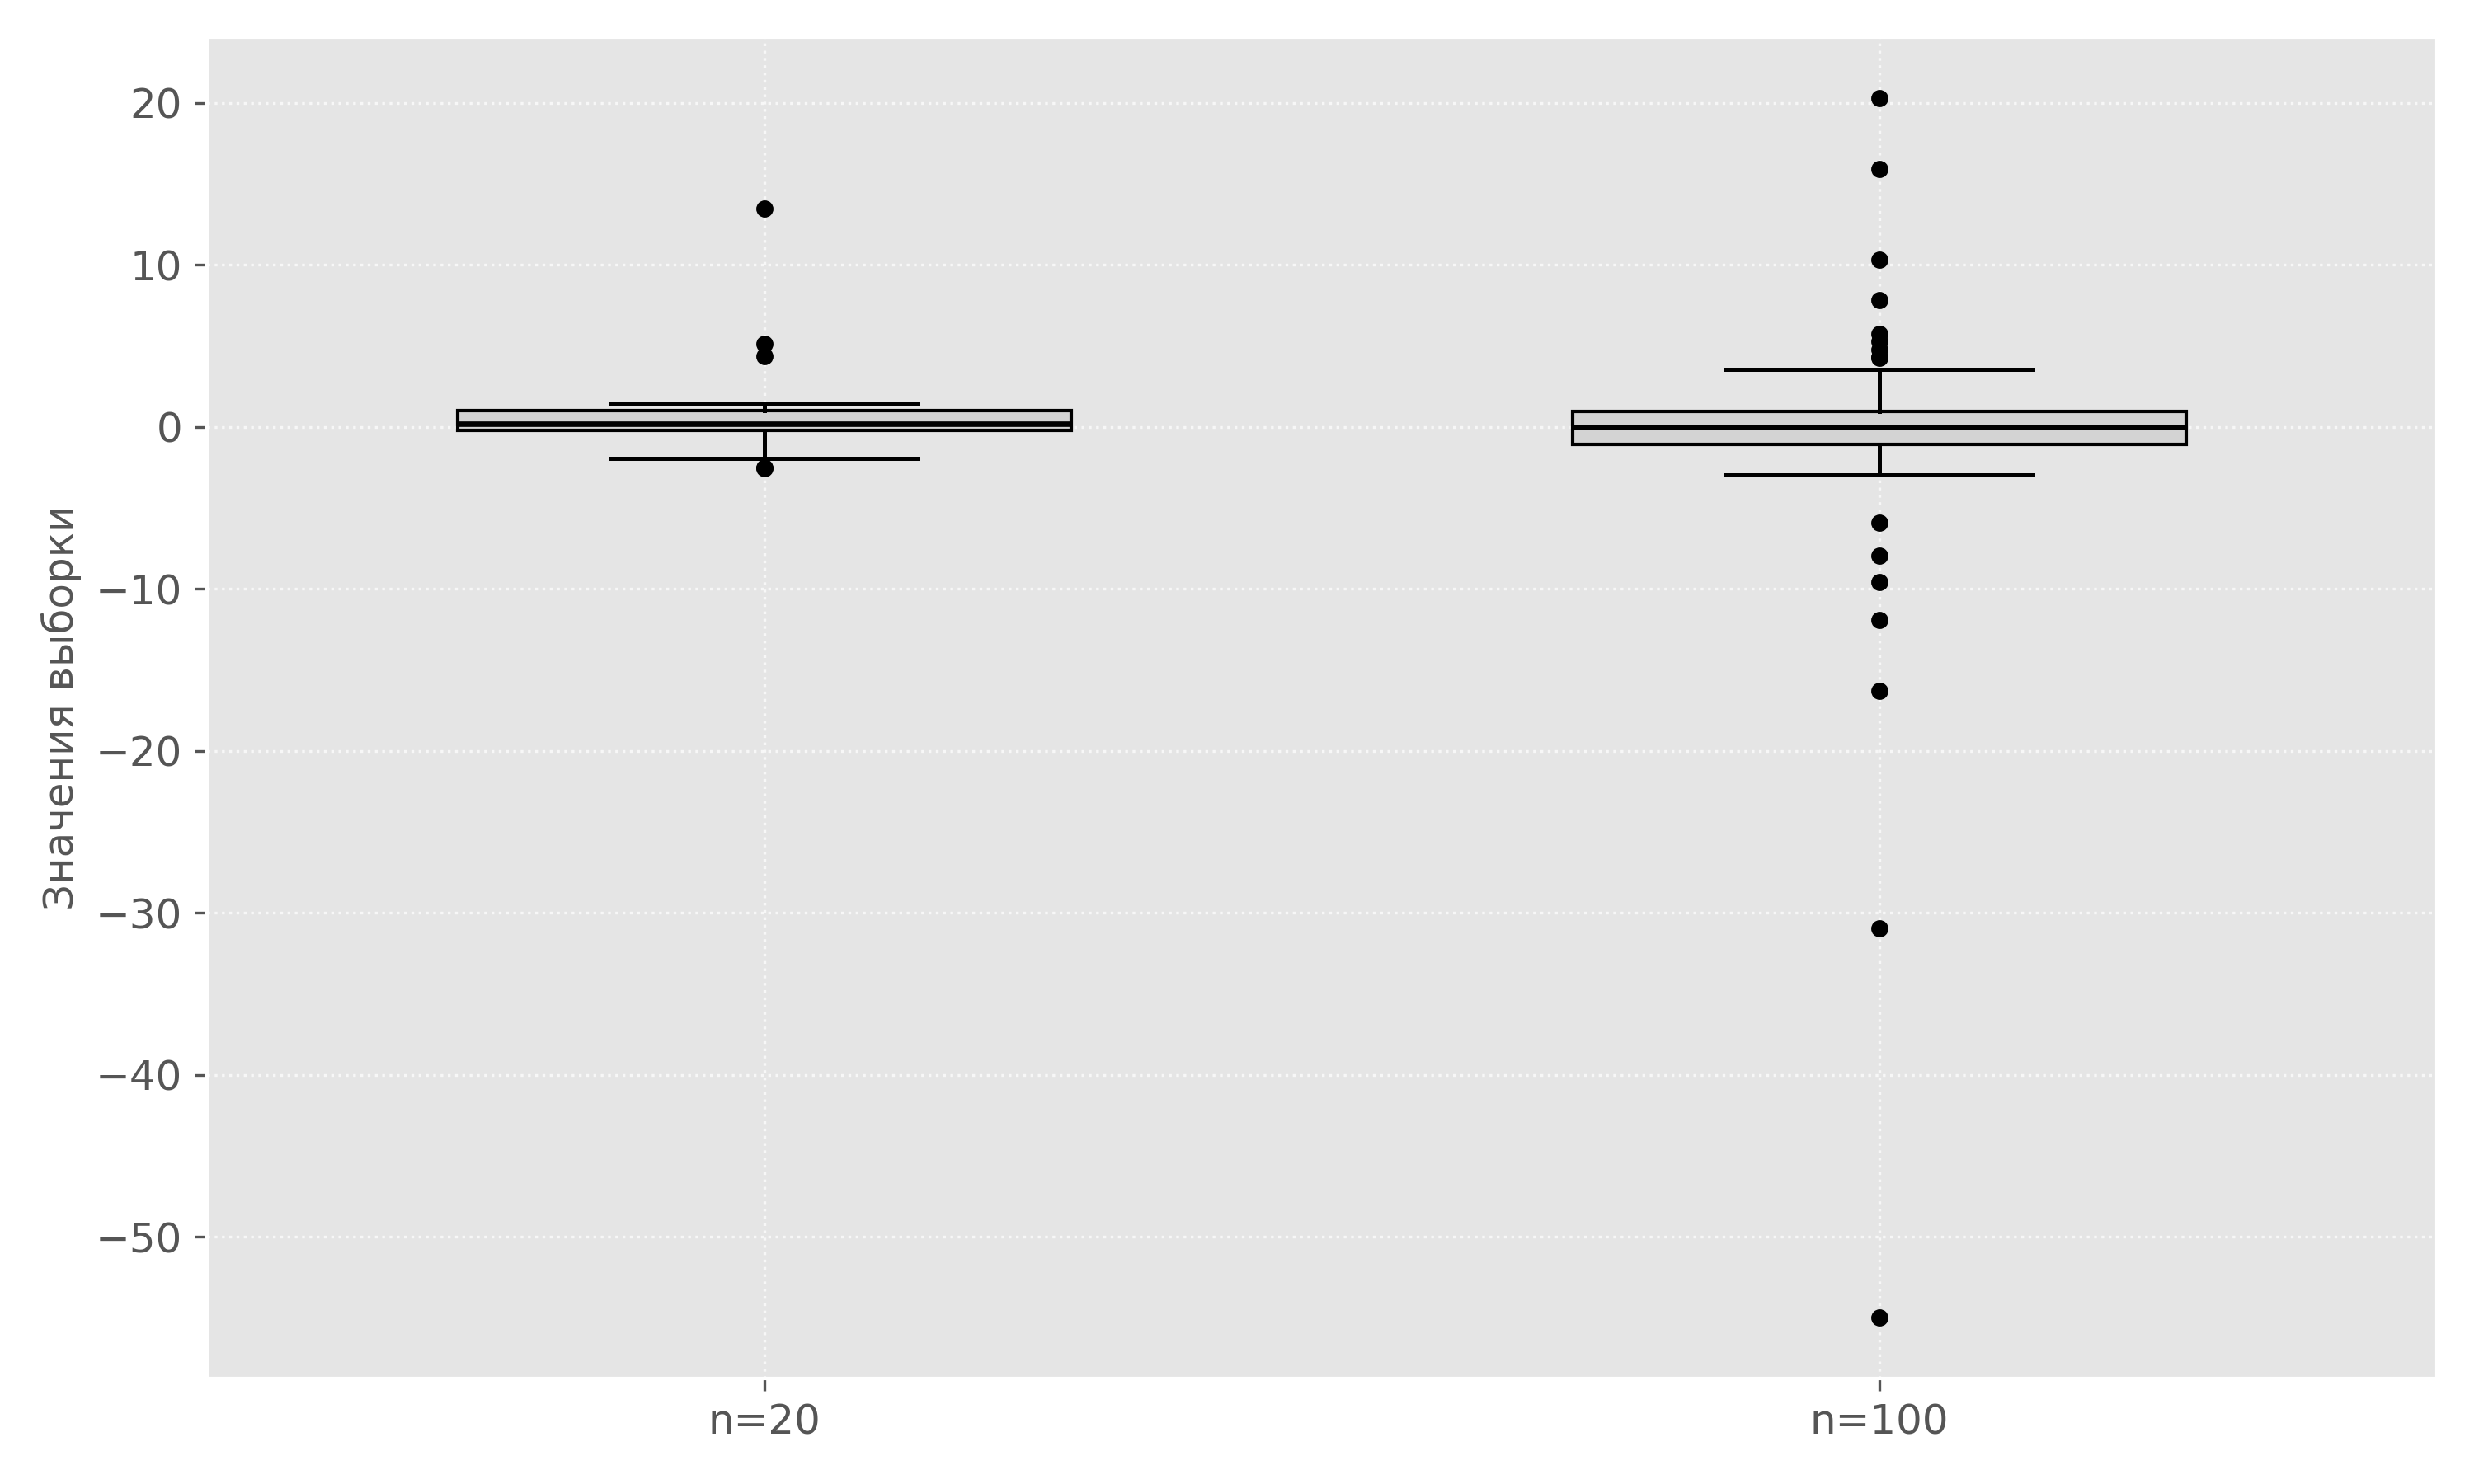
\includegraphics[width=\textwidth]{../figures/cauchy_boxplot.png}
    \caption{Боксплот Тьюки для распределения Коши $C(0,1)$}
    \label{fig:cauchy_boxplot}
\end{figure}

\begin{figure}[H]
    \centering
    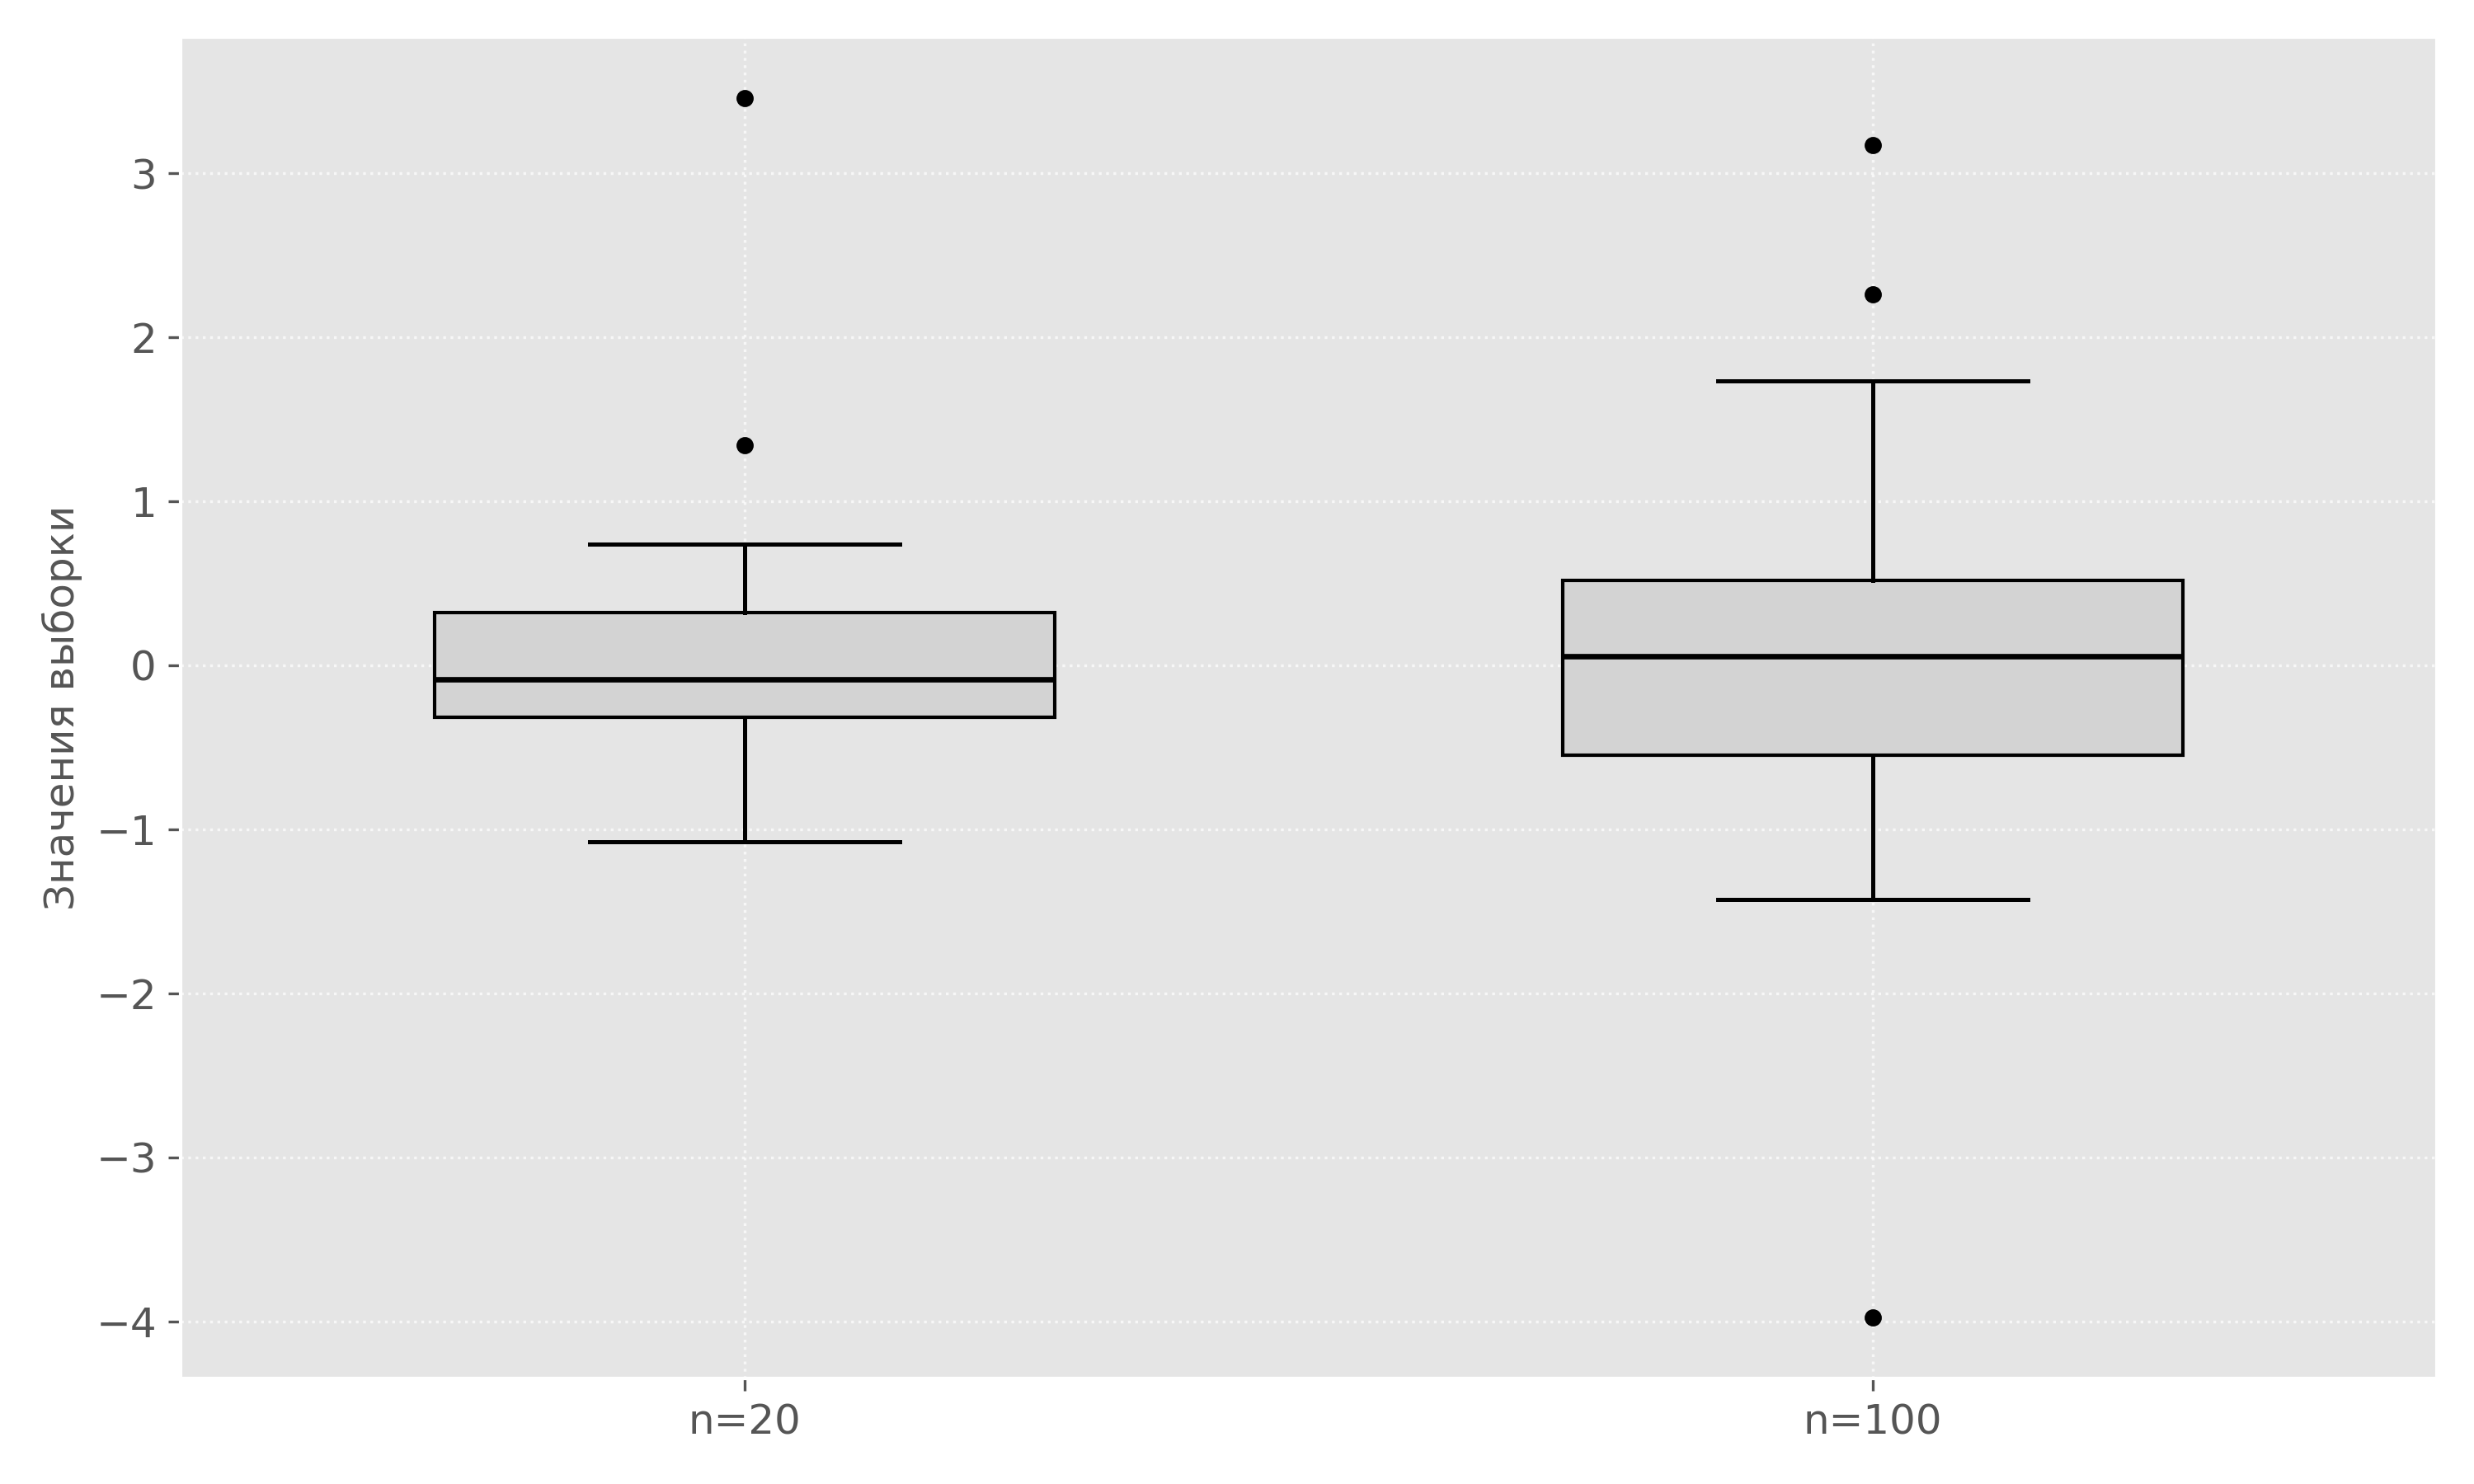
\includegraphics[width=\textwidth]{../figures/laplace_boxplot.png}
    \caption{Боксплот Тьюки для распределения Лапласа $L(0, 1/\sqrt{2})$}
    \label{fig:laplace_boxplot}
\end{figure}

\begin{figure}[H]
    \centering
    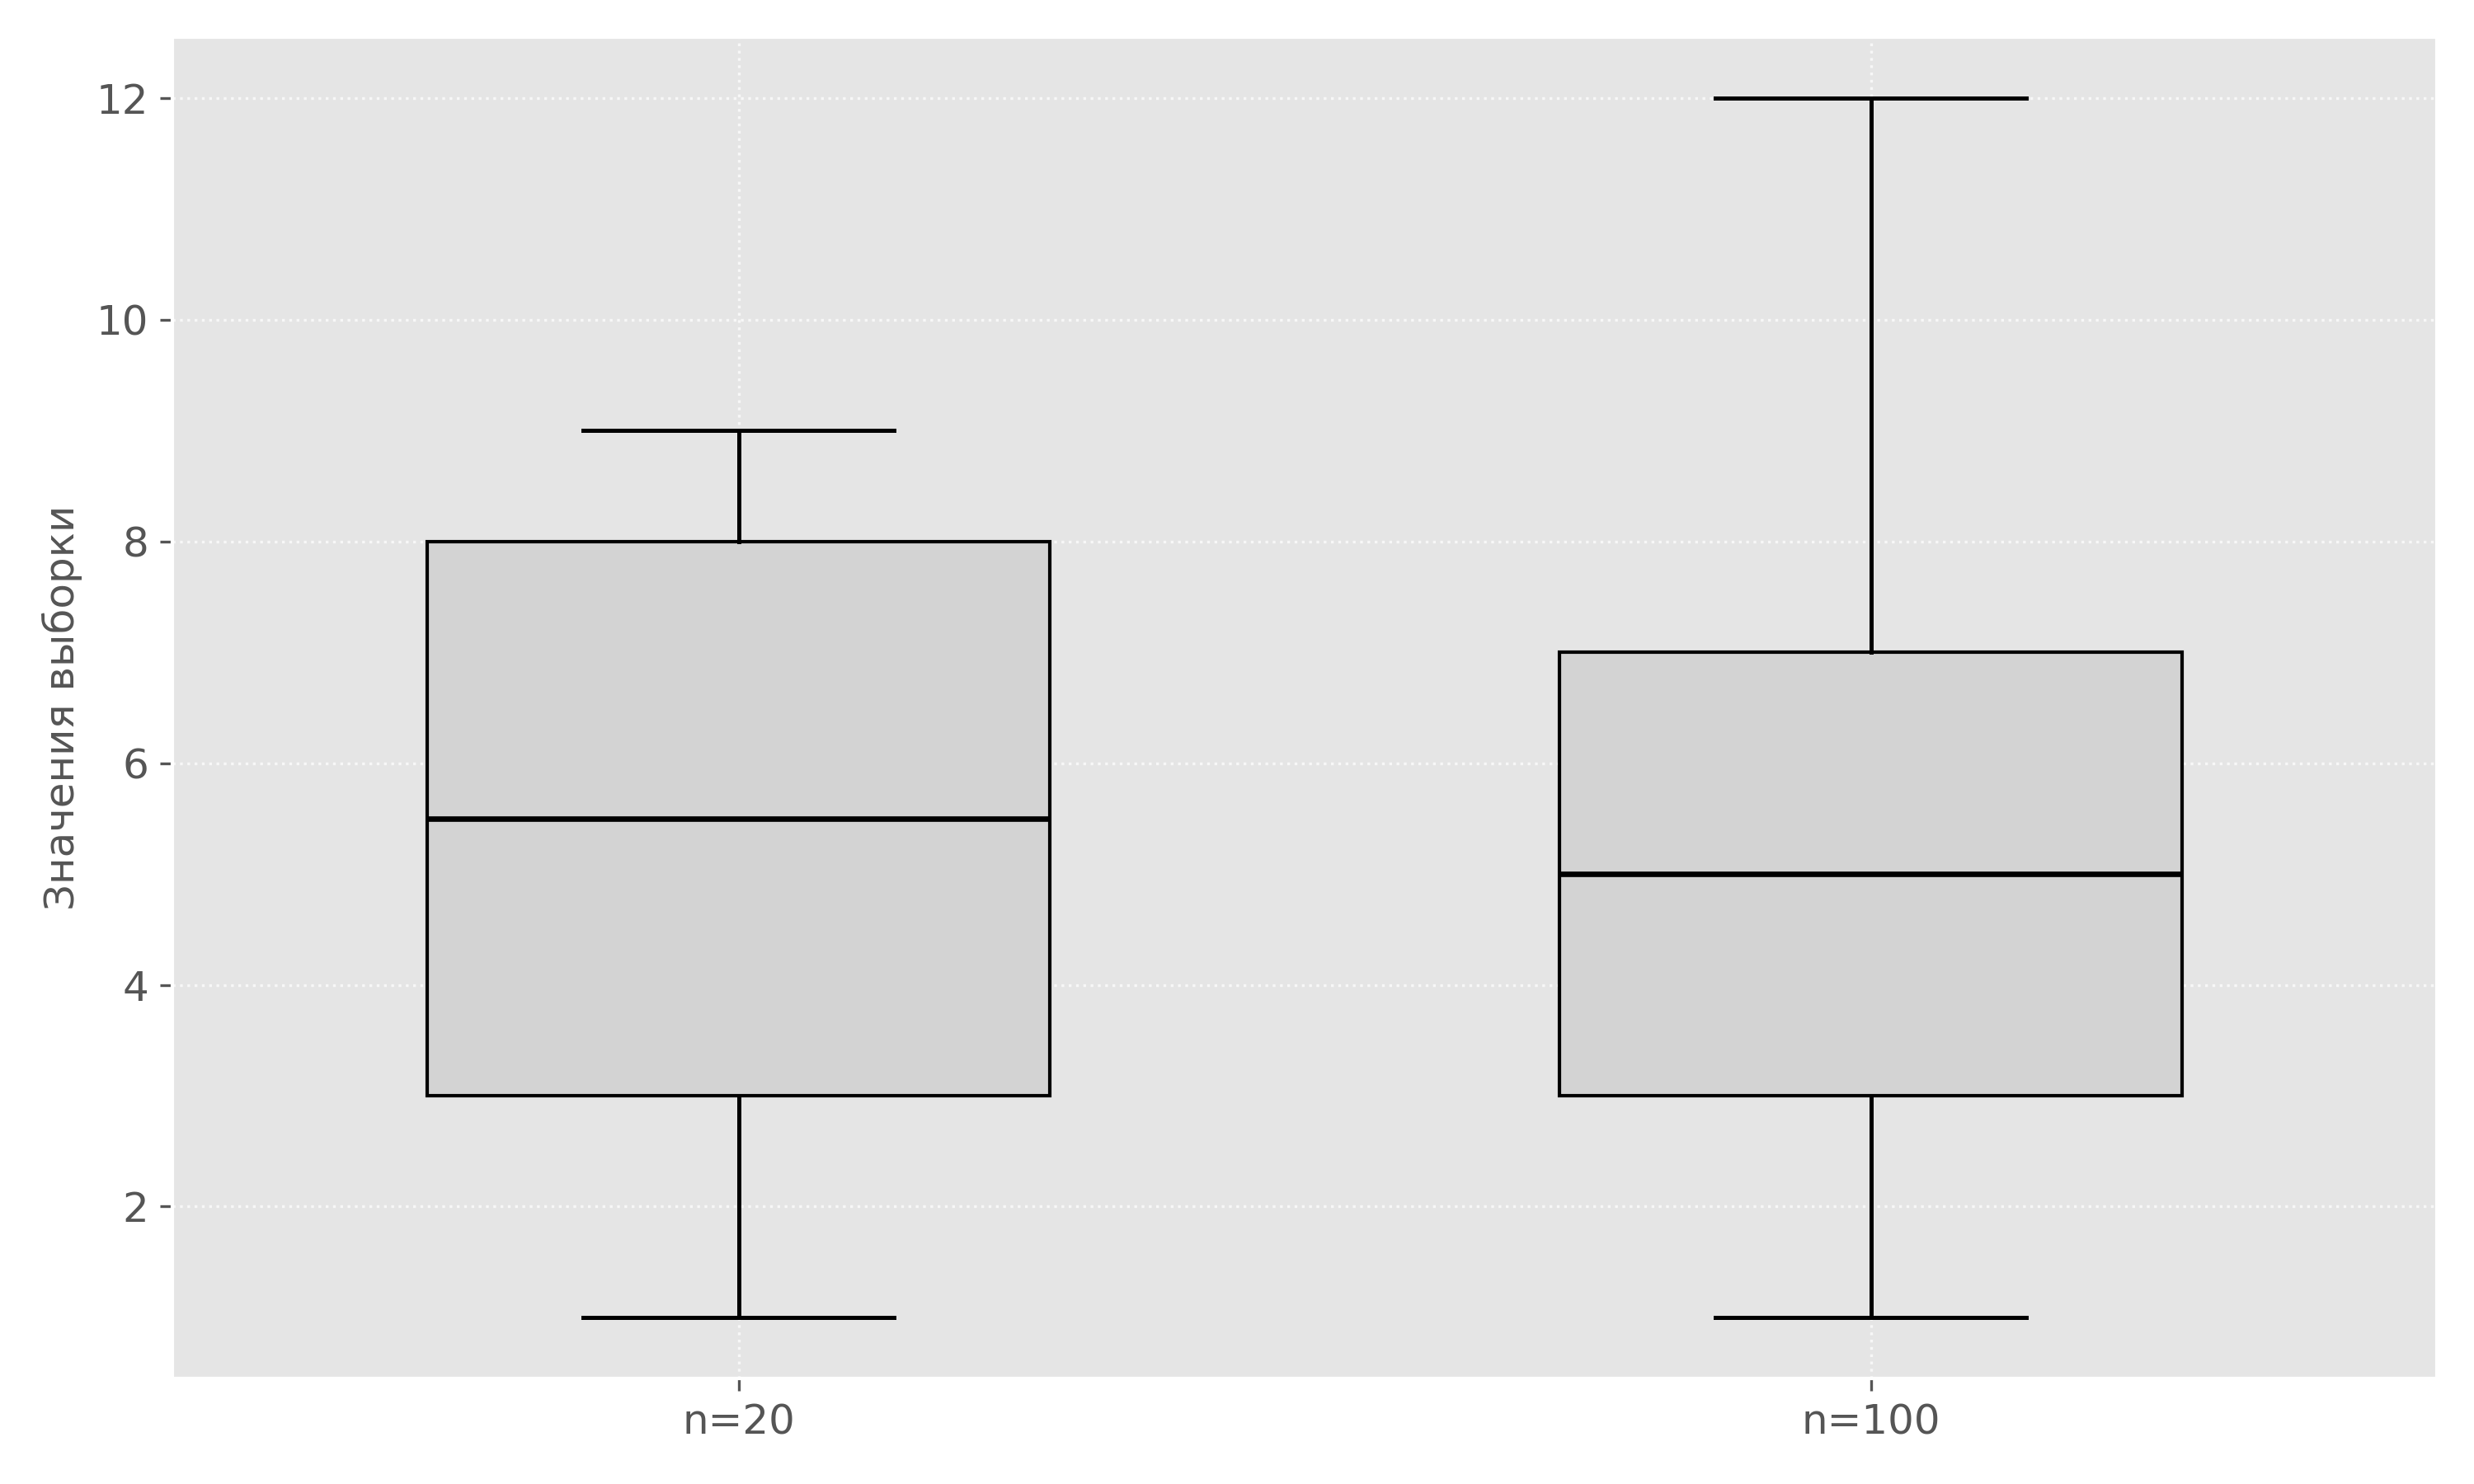
\includegraphics[width=\textwidth]{../figures/poisson_boxplot.png}
    \caption{Боксплот Тьюки для распределения Пуассона $P(5)$}
    \label{fig:poisson_boxplot}
\end{figure}

\begin{figure}[H]
    \centering
    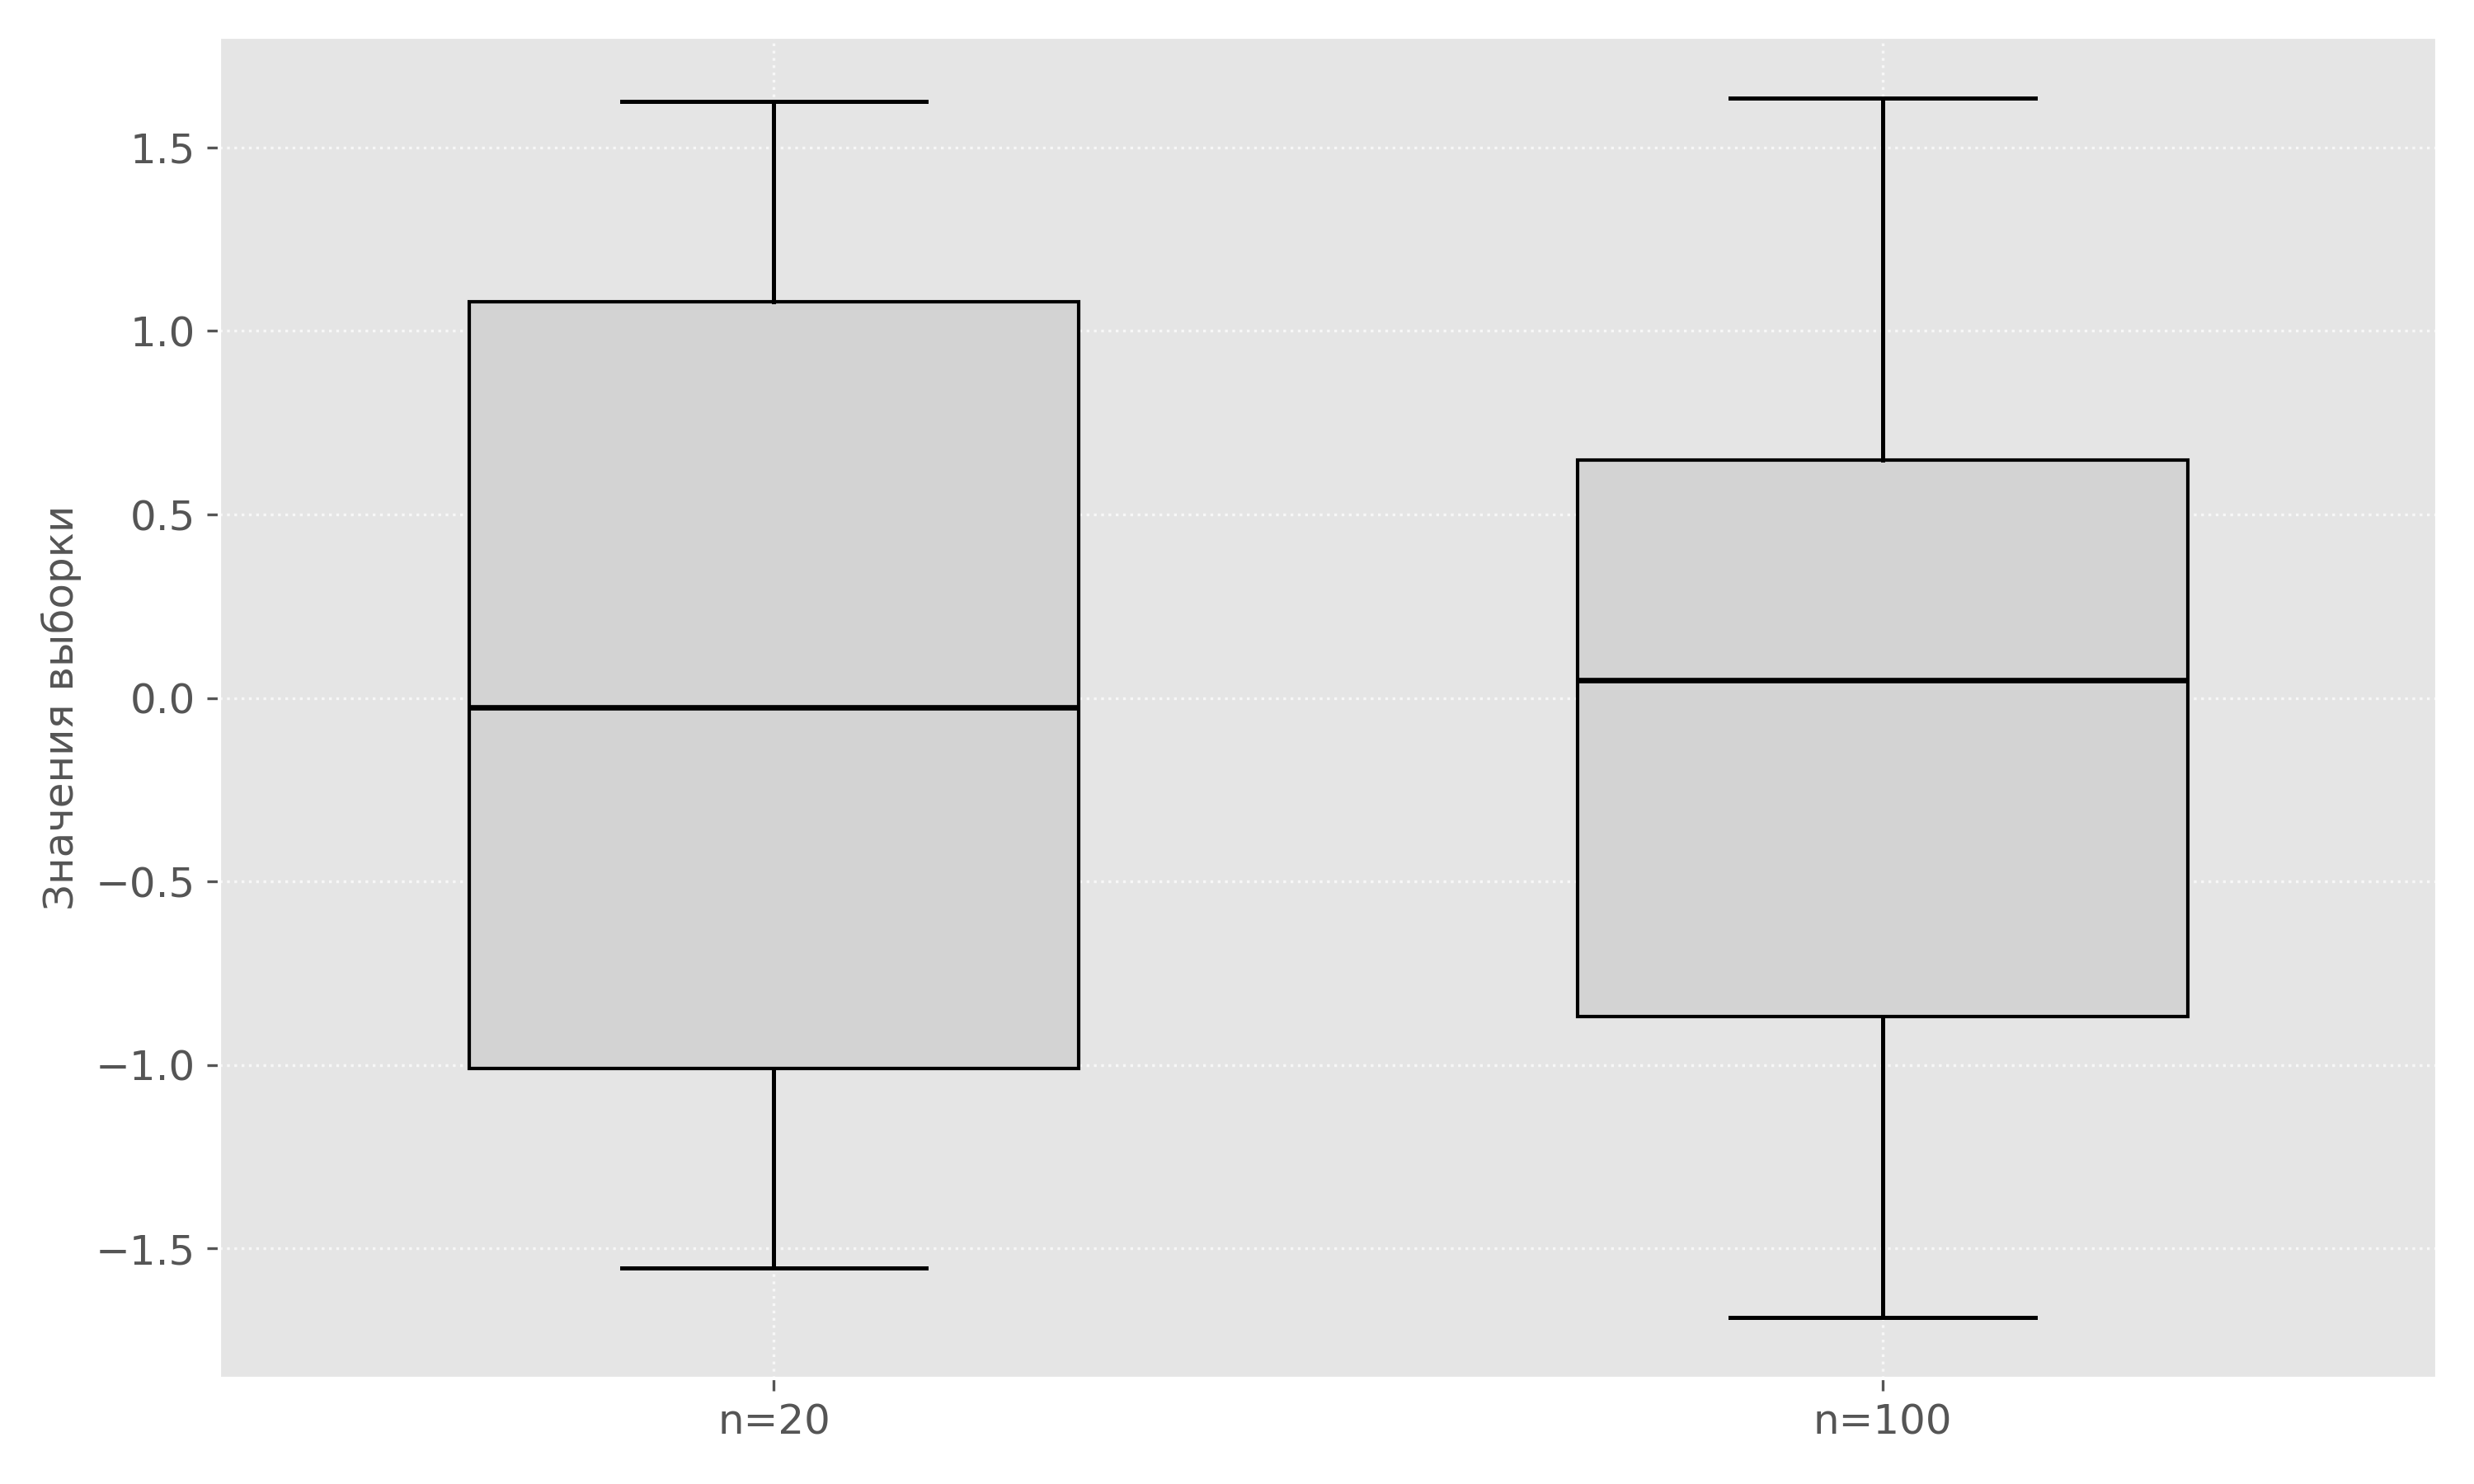
\includegraphics[width=\textwidth]{../figures/uniform_boxplot.png}
    \caption{Боксплот Тьюки для равномерного распределения $U(-\sqrt{3}, \sqrt{3})$}
    \label{fig:uniform_boxplot}
\end{figure}

\begin{figure}[H]
    \centering
    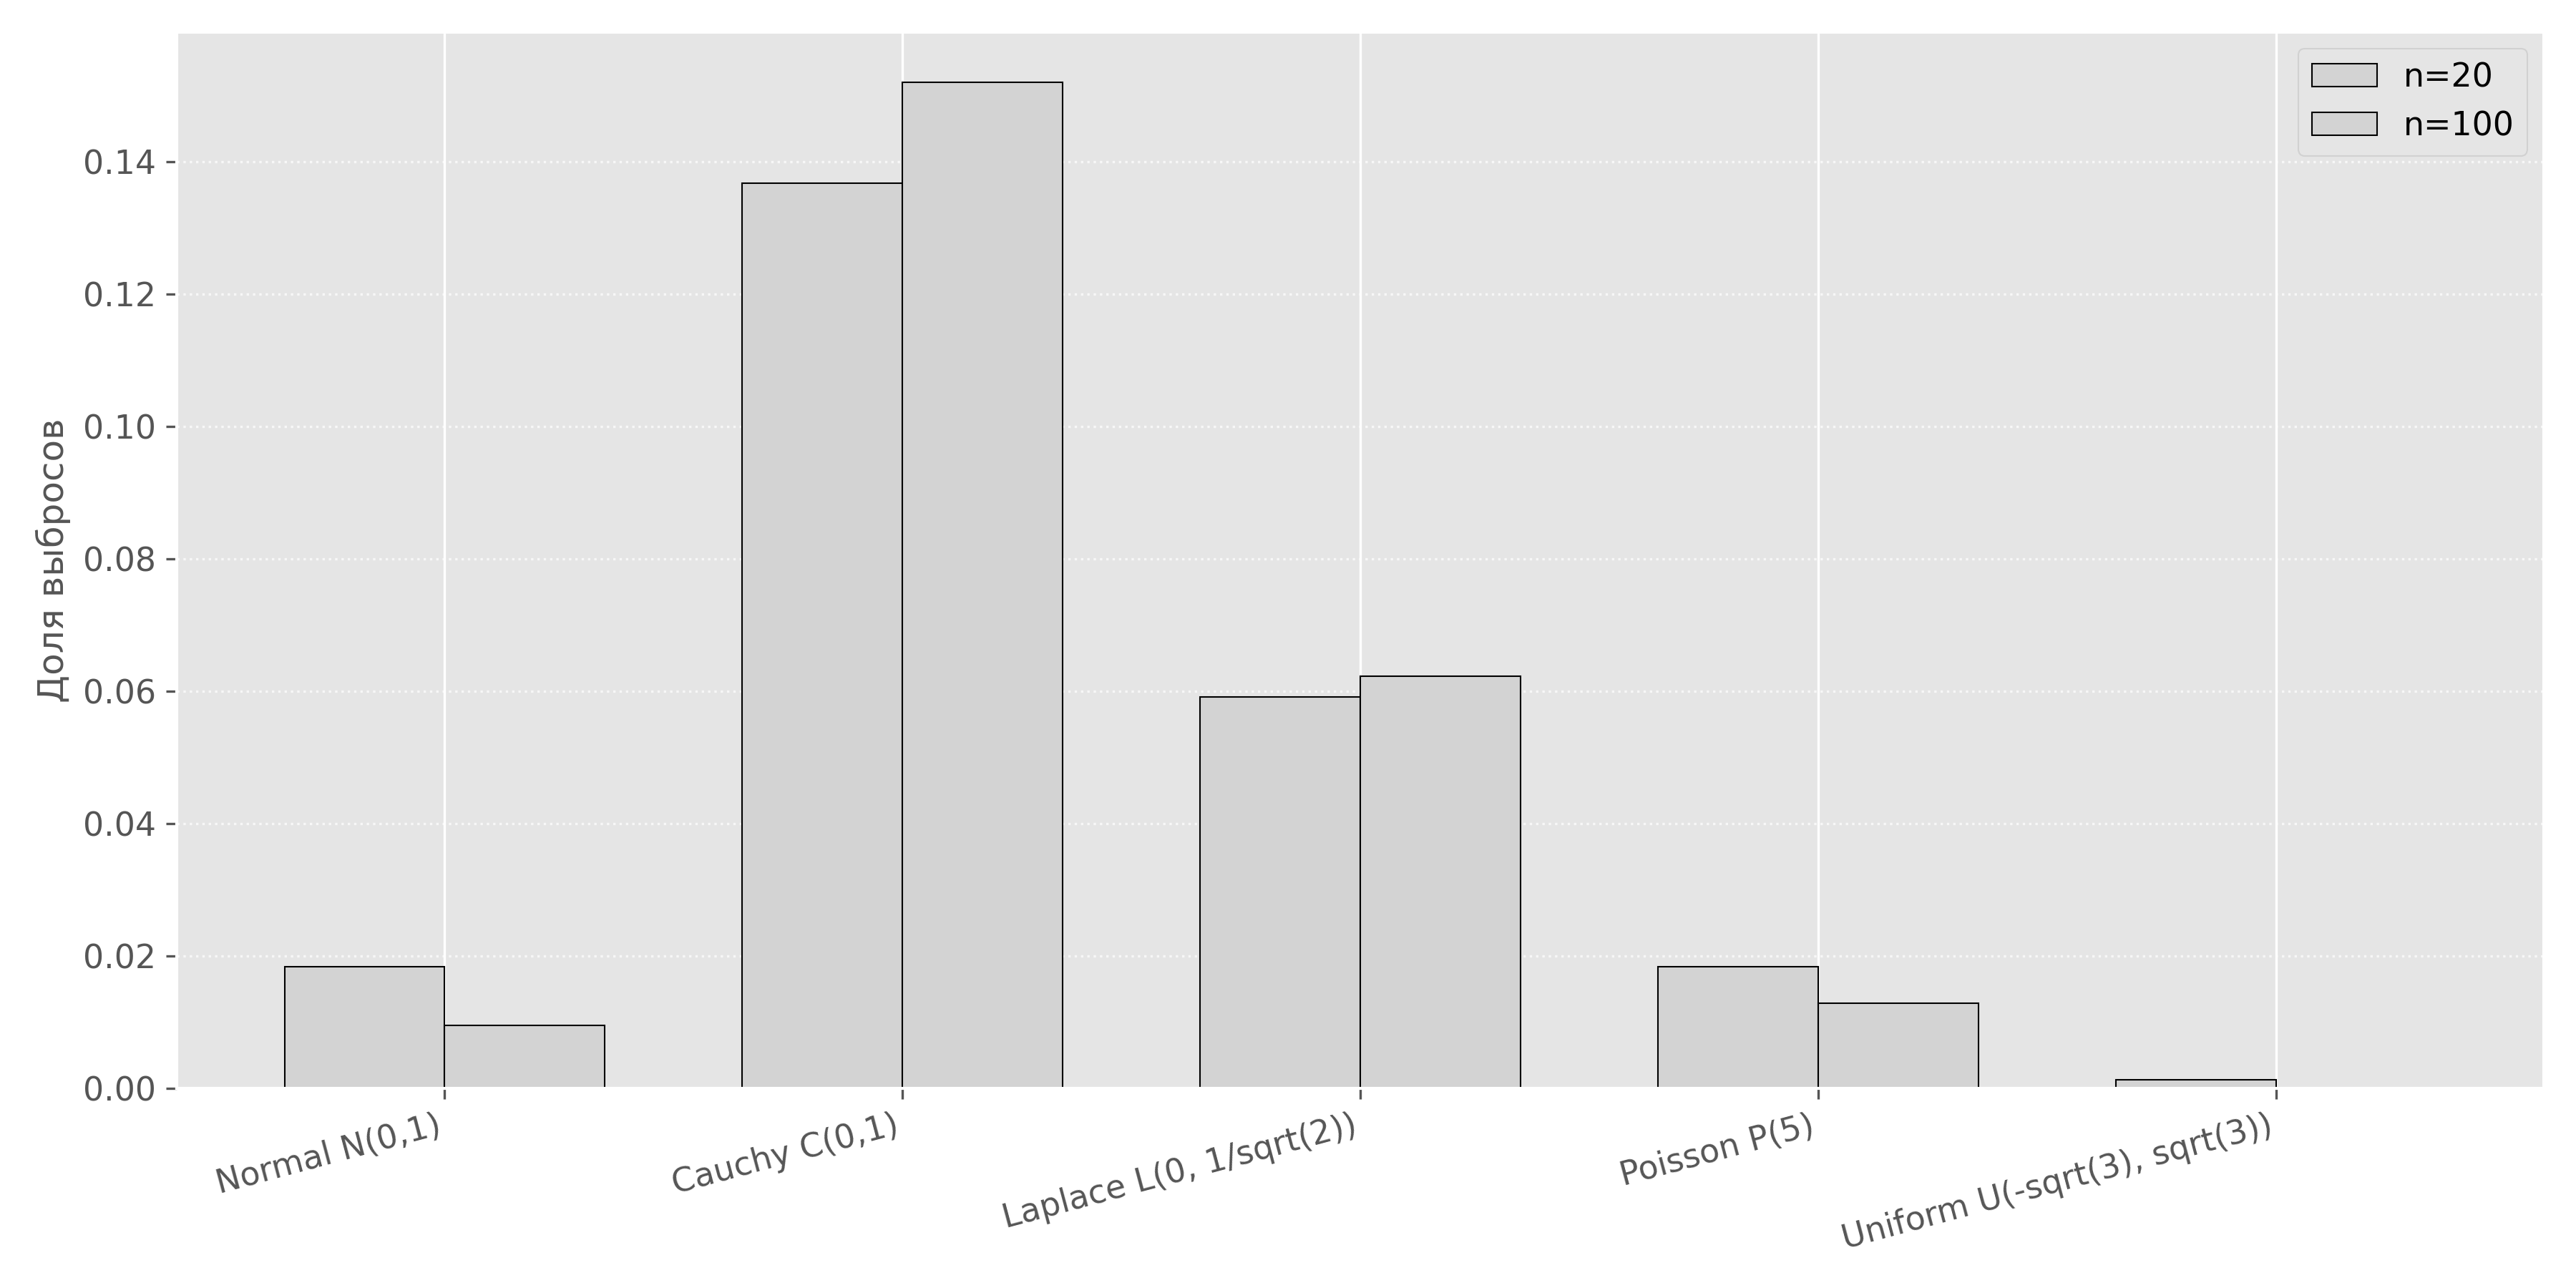
\includegraphics[width=\textwidth]{../figures/outlier_share.png}
    \caption{Сравнение средних долей выбросов по правилу Тьюки}
    \label{fig:outlier_share}
\end{figure}

\section{Обсуждение}

Анализ эмпирических долей выбросов выявляет жесткую зависимость между формой хвостов распределения и количеством генерируемых аномалий.

Для равномерного распределения $U(-\sqrt{3}, \sqrt{3})$ с конечным носителем плотности появление значений за аналитическими границами усов Тьюки теоретически невозможно. Экспериментальные данные строго подтверждают этот факт: при $n=100$ доля выбросов равна $0.000$. Фиксация единичных аномалий на уровне $0.001$ при $n=20$ является вычислительным артефактом. Она вызвана случайным сужением выборочной интерквартильной широты $IQR$ на микровыборках, а не свойствами самого закона распределения.

Распределения с экспоненциальным убыванием плотности вероятности (нормальное $N(0, 1)$ и дискретное Пуассона $P(5)$) характеризуются минимальной долей выбросов. При увеличении объема выборки до $n=100$ эмпирическая доля аномалий для нормального закона составляет $0.010$, для пуассоновского — $0.013$. С ростом $n$ оценка стабилизируется, нивелируя влияние случайных флуктуаций $IQR$.

Распределение Лапласа $L(0, 1/\sqrt{2})$ обладает более тяжелыми хвостами по сравнению с нормальным законом. Это обуславливает кратное увеличение числа аномальных наблюдений: эмпирическая доля выбросов составляет $0.059$ при $n=20$ и возрастает до $0.062$ при $n=100$.

Максимальное количество аномалий генерирует распределение Коши $C(0, 1)$ за счет степенного характера убывания плотности и отсутствия конечных теоретических моментов. Расчетная доля выбросов для данного закона достигает $0.152$ ($15.2\%$) при $n=100$. Цифры доказывают недопустимость применения классических неробастных методов для обработки выборок Коши.

\section{Выводы}

В ходе работы исследовано влияние формы распределения и объема выборки на вероятность появления аномальных значений при графическом анализе одномерных данных боксплотом Тьюки. 

Для законов с финитным носителем (Равномерное) генерация выбросов при достаточных объемах выборки исключена. Распределения с тяжелыми хвостами (Коши) систематически производят более $15\%$ аномалий независимо от мощности выборки, что диктует необходимость применения робастных статистических оценок при их исследовании.

Рост объема выборки от $n=20$ до $n=100$ обеспечивает стабилизацию выборочной интерквартильной широты $IQR$, за счет чего эмпирическая доля выбросов сходится к истинной теоретической вероятности выхода случайной величины за границы нормального разброса для заданного закона распределения.

\refstepcounter{section}
\addcontentsline{toc}{section}{\thesection\ Список литературы}
\renewcommand{\refname}{\thesection\ Список литературы}

\begin{thebibliography}{9}

    \bibitem{babakhina}
    Бабахина С. А., Баженов А. Н. Практикум по математической статистике: учеб. пособие. — СПб. : Санкт-Петербургский политехнический университет Петра Великого, 2026. 

    \bibitem{maksimov}
    Максимов Ю. Д. Математика. Теория и практика по математической статистике. Конспект-справочник по теории вероятностей : учеб. пособие. — СПб. : Изд-во Политехн. ун-та, 2009. — 395 с. 

\end{thebibliography}

\section{Приложение}

Исходный код программ доступен в репозитории на GitHub: \\
\url{https://github.com/Reichenau/math-stats-labs}
 
\end{document}
